from pathlib import Path
import shutil, zipfile

base = Path("/mnt/data/robotmanip_report")
fig_dir = base/"figures"
base.mkdir(exist_ok=True)
fig_dir.mkdir(exist_ok=True)

# copy extracted figs we want
src_figs = Path("/mnt/data/robotmanip_figs")
keep = ["s02_img01.png","s02_img02.jpg","s05_img01.png","s05_img02.png","s05_img03.png"]
for fn in keep:
    shutil.copy2(src_figs/fn, fig_dir/fn)

tex = r"""
% Compile with: lualatex report.tex  (recommended)
\documentclass[a4paper,11pt]{ltjsarticle}

\usepackage{amsmath,amssymb}
\usepackage{graphicx}
\usepackage{booktabs}
\usepackage{siunitx}
\usepackage{hyperref}
\usepackage{caption}
\usepackage{subcaption}
\usepackage[margin=25mm]{geometry}

\graphicspath{{figures/}}

\title{複数の逆運動学（IK）計算手法によるロボットアーム制御の比較\\
\large --- DOBOT Magician E6（ROS/Gazebo）シミュレーション ---}
\author{（M3）Liao Ciou-fen \quad（M1）Clement Lai Jian Sheng \quad（M1）飯田 尚昭 \quad（M1）奥 朋哉}
\date{\today}

\begin{document}
\maketitle

\begin{abstract}
本レポートでは，ROS/Gazebo 上で 6 軸ロボットアーム（DOBOT Magician E6）を用い，
複数の逆運動学（Inverse Kinematics: IK）ソルバの挙動差を比較した．
到達可能領域内にランダムに設定した 20 個の目標点に対し，
Trac-IK，Orocos KDL の Newton--Raphson 法（KDL-NR），および関節角制限付き（KDL-NR\_JL）を用いて
エンドエフェクタを追従させ，位置誤差・所要時間・到達成功数を評価した．
結果として，ソルバ・初期姿勢条件により収束性や失敗様式が大きく異なることを確認した．
\end{abstract}

\section{背景}
ロボットアームの先端（エンドエフェクタ）を所望の位置・姿勢へ到達させるために，
逆運動学（IK）は基本的な要素技術である．
一方で，IK の数値解法は初期値・特異点近傍・関節角制限などの条件に強く影響され，
同一タスクでもソルバにより収束性・計算時間・精度が大きく変化し得る．
本研究では，ROS/Gazebo 環境において複数 IK 手法を同条件で比較し，
挙動差と失敗パターンを整理することを目的とする．

\section{対象システムと実験設定}
\subsection{シミュレーション環境とモデル}
シミュレーションは ROS/Gazebo を用い，6 軸ロボットアーム DOBOT Magician E6 を対象とした．fileciteturn1file0L3-L5
図\ref{fig:dobot}にロボット外観例を示す．

\begin{figure}[h]
  \centering
  \begin{subfigure}[t]{0.48\linewidth}
    \centering
    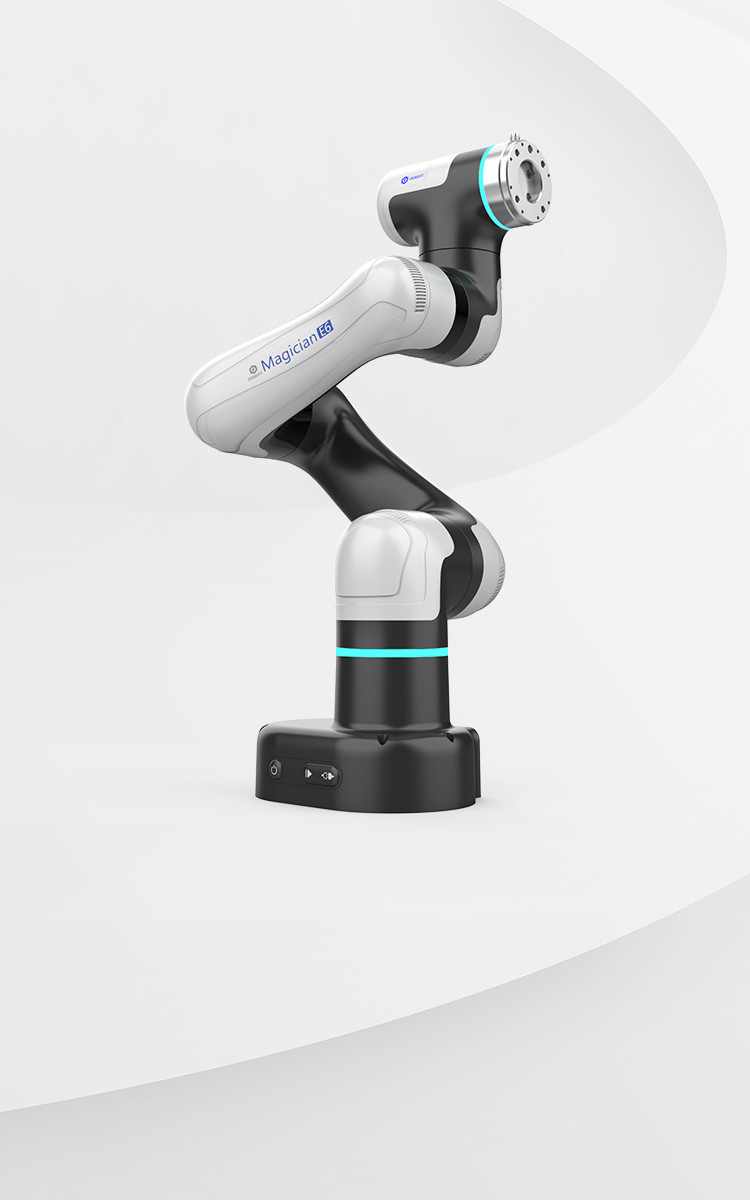
\includegraphics[width=\linewidth]{s02_img01.png}
    \caption{DOBOT Magician E6 外観（例）}
  \end{subfigure}
  \begin{subfigure}[t]{0.48\linewidth}
    \centering
    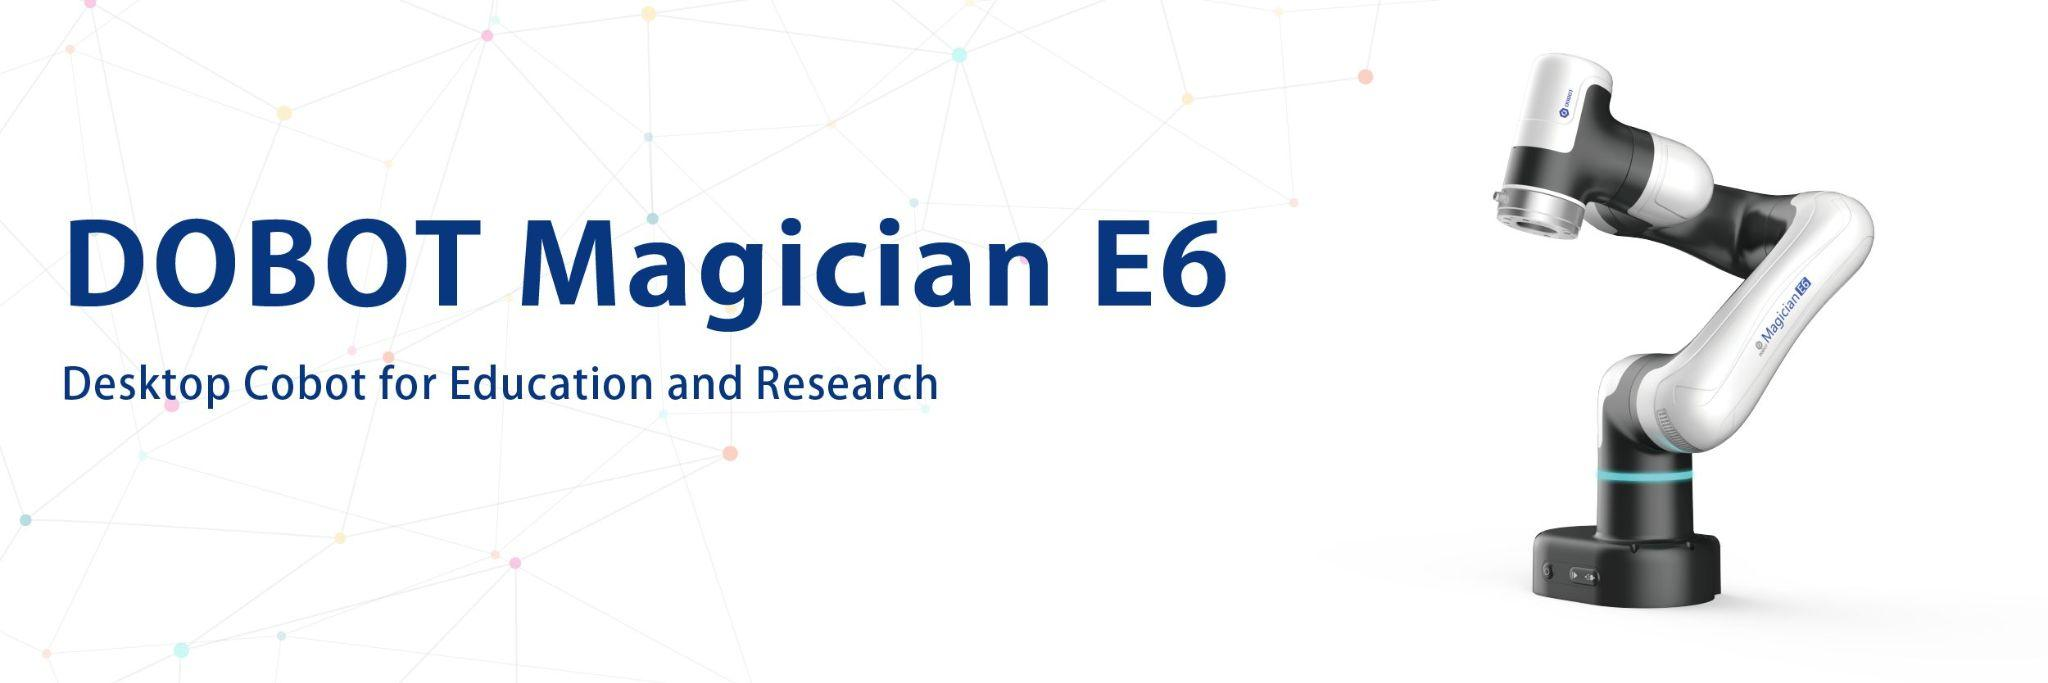
\includegraphics[width=\linewidth]{s02_img02.jpg}
    \caption{製品紹介スライド画像（例）}
  \end{subfigure}
  \caption{シミュレーション対象ロボットの例}
  \label{fig:dobot}
\end{figure}

\subsection{タスク（目標点追従）}
到達可能領域内に 20 個の目標点をランダムに生成し，
Gazebo 空間内に赤点としてスポーンさせた上で，先端リンクが順次到達するよう制御した．fileciteturn1file0L7-L12
評価指標として，(i) 位置誤差，(ii) 所要時間，(iii) 到達成功数を用い，
さらに初期姿勢（初期関節角）を変えた条件でも比較した．fileciteturn1file0L11-L12

\section{比較した IK 手法}
本比較で用いた IK ソルバを表\ref{tab:ik}に示す．fileciteturn1file0L7-L9

\begin{table}[h]
  \centering
  \caption{比較した IK ソルバ}
  \label{tab:ik}
  \begin{tabular}{lll}
    \toprule
    名称 & 実装/パッケージ & 概要 \\
    \midrule
    Trac-IK & ROS IK solver package & IK を高速・高ロバストに解くことを狙った手法 \\
    KDL-NR & Orocos KDL & Newton--Raphson による数値 IK（関節角制限なし）\\
    KDL-NR\_JL & Orocos KDL & Newton--Raphson + 関節角制限（Joint Limit）\\
    \bottomrule
  \end{tabular}
\end{table}

\section{結果}
図\ref{fig:results}に，各手法の目標値（target）と先端位置（ee\_pose）の $x,y,z$ 軸方向の推移，
および位置誤差（例：絶対距離）を示す．fileciteturn1file0L16-L22
横軸の幅がタスク全体の所要時間を表し，
例として Trac-IK で約 70\,s，KDL 系で約 16\,s のケースが示されている．fileciteturn1file0L19-L22

\begin{figure}[h]
  \centering
  \begin{subfigure}[t]{0.98\linewidth}
    \centering
    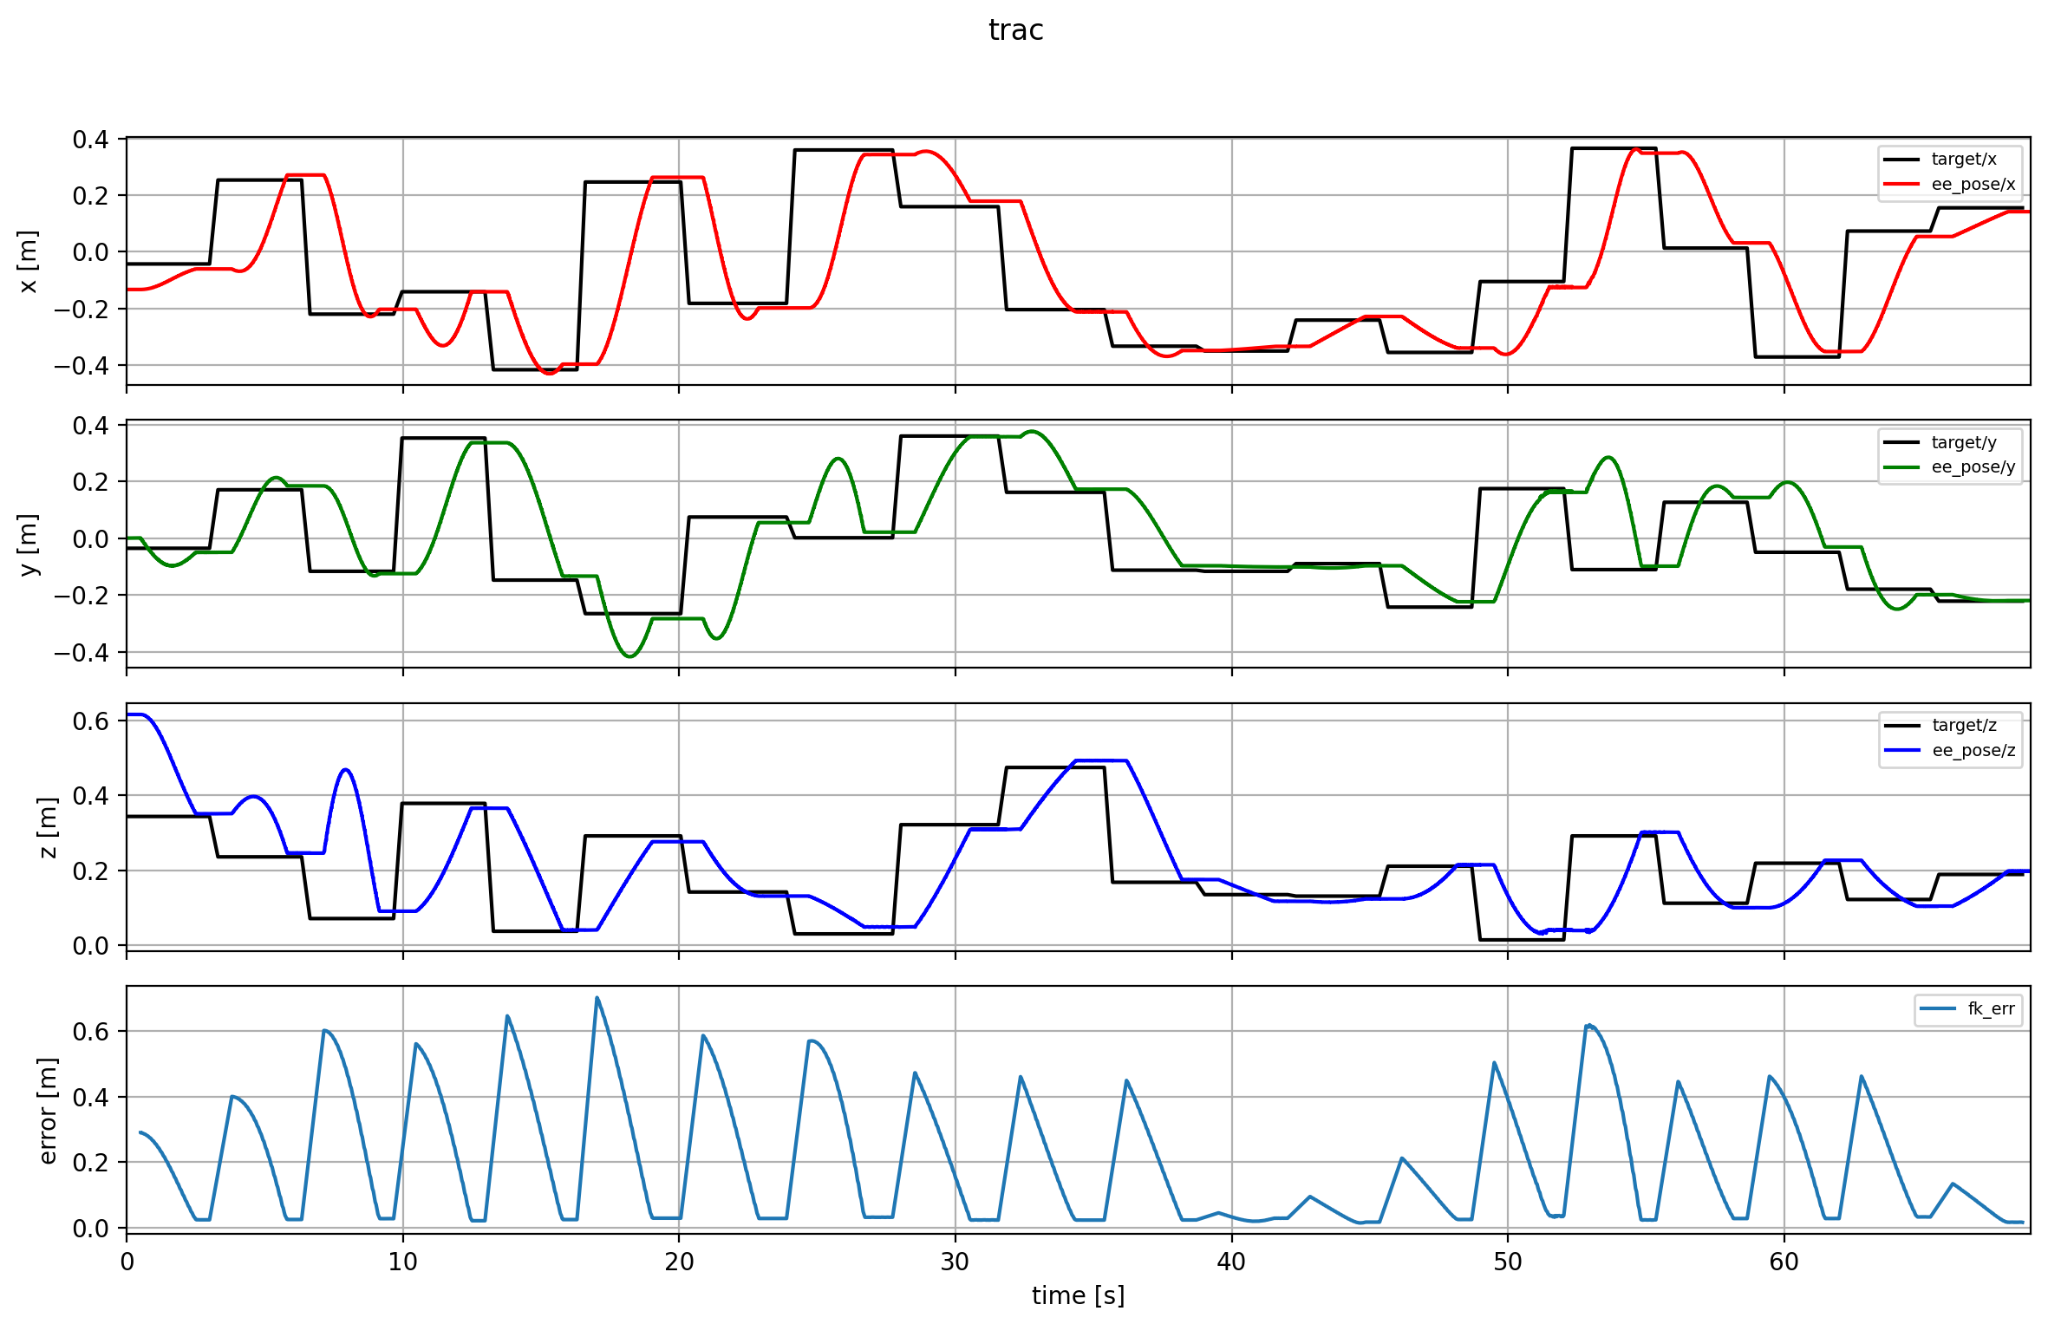
\includegraphics[width=\linewidth]{s05_img01.png}
    \caption{Trac-IK の例（目標値と追従，誤差）}
  \end{subfigure}

  \vspace{1em}

  \begin{subfigure}[t]{0.98\linewidth}
    \centering
    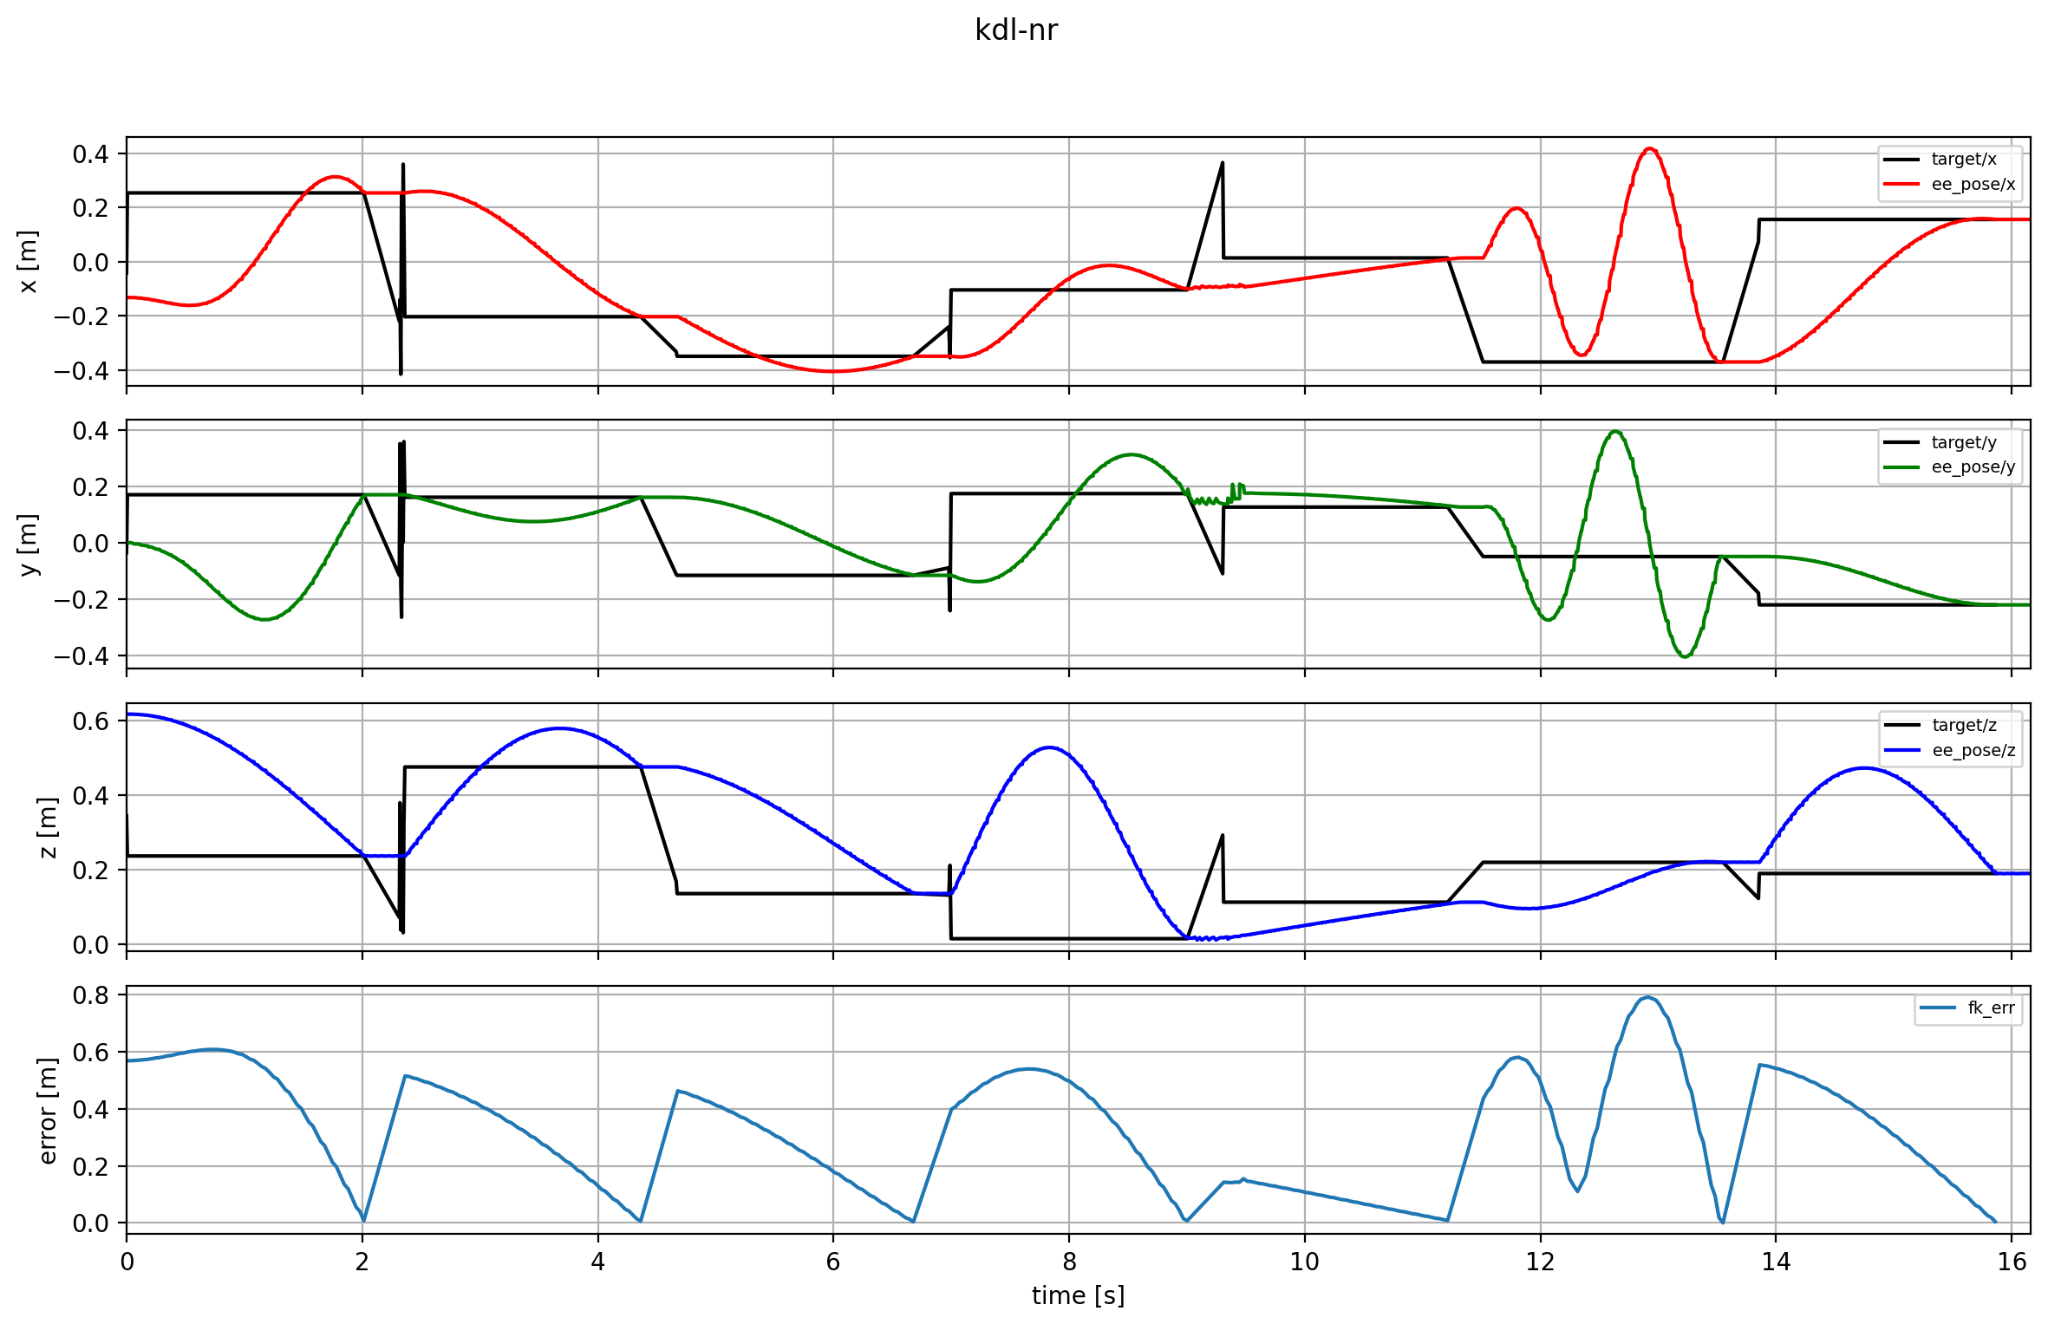
\includegraphics[width=\linewidth]{s05_img02.png}
    \caption{KDL-NR の例（目標値と追従，誤差）}
  \end{subfigure}

  \vspace{1em}

  \begin{subfigure}[t]{0.98\linewidth}
    \centering
    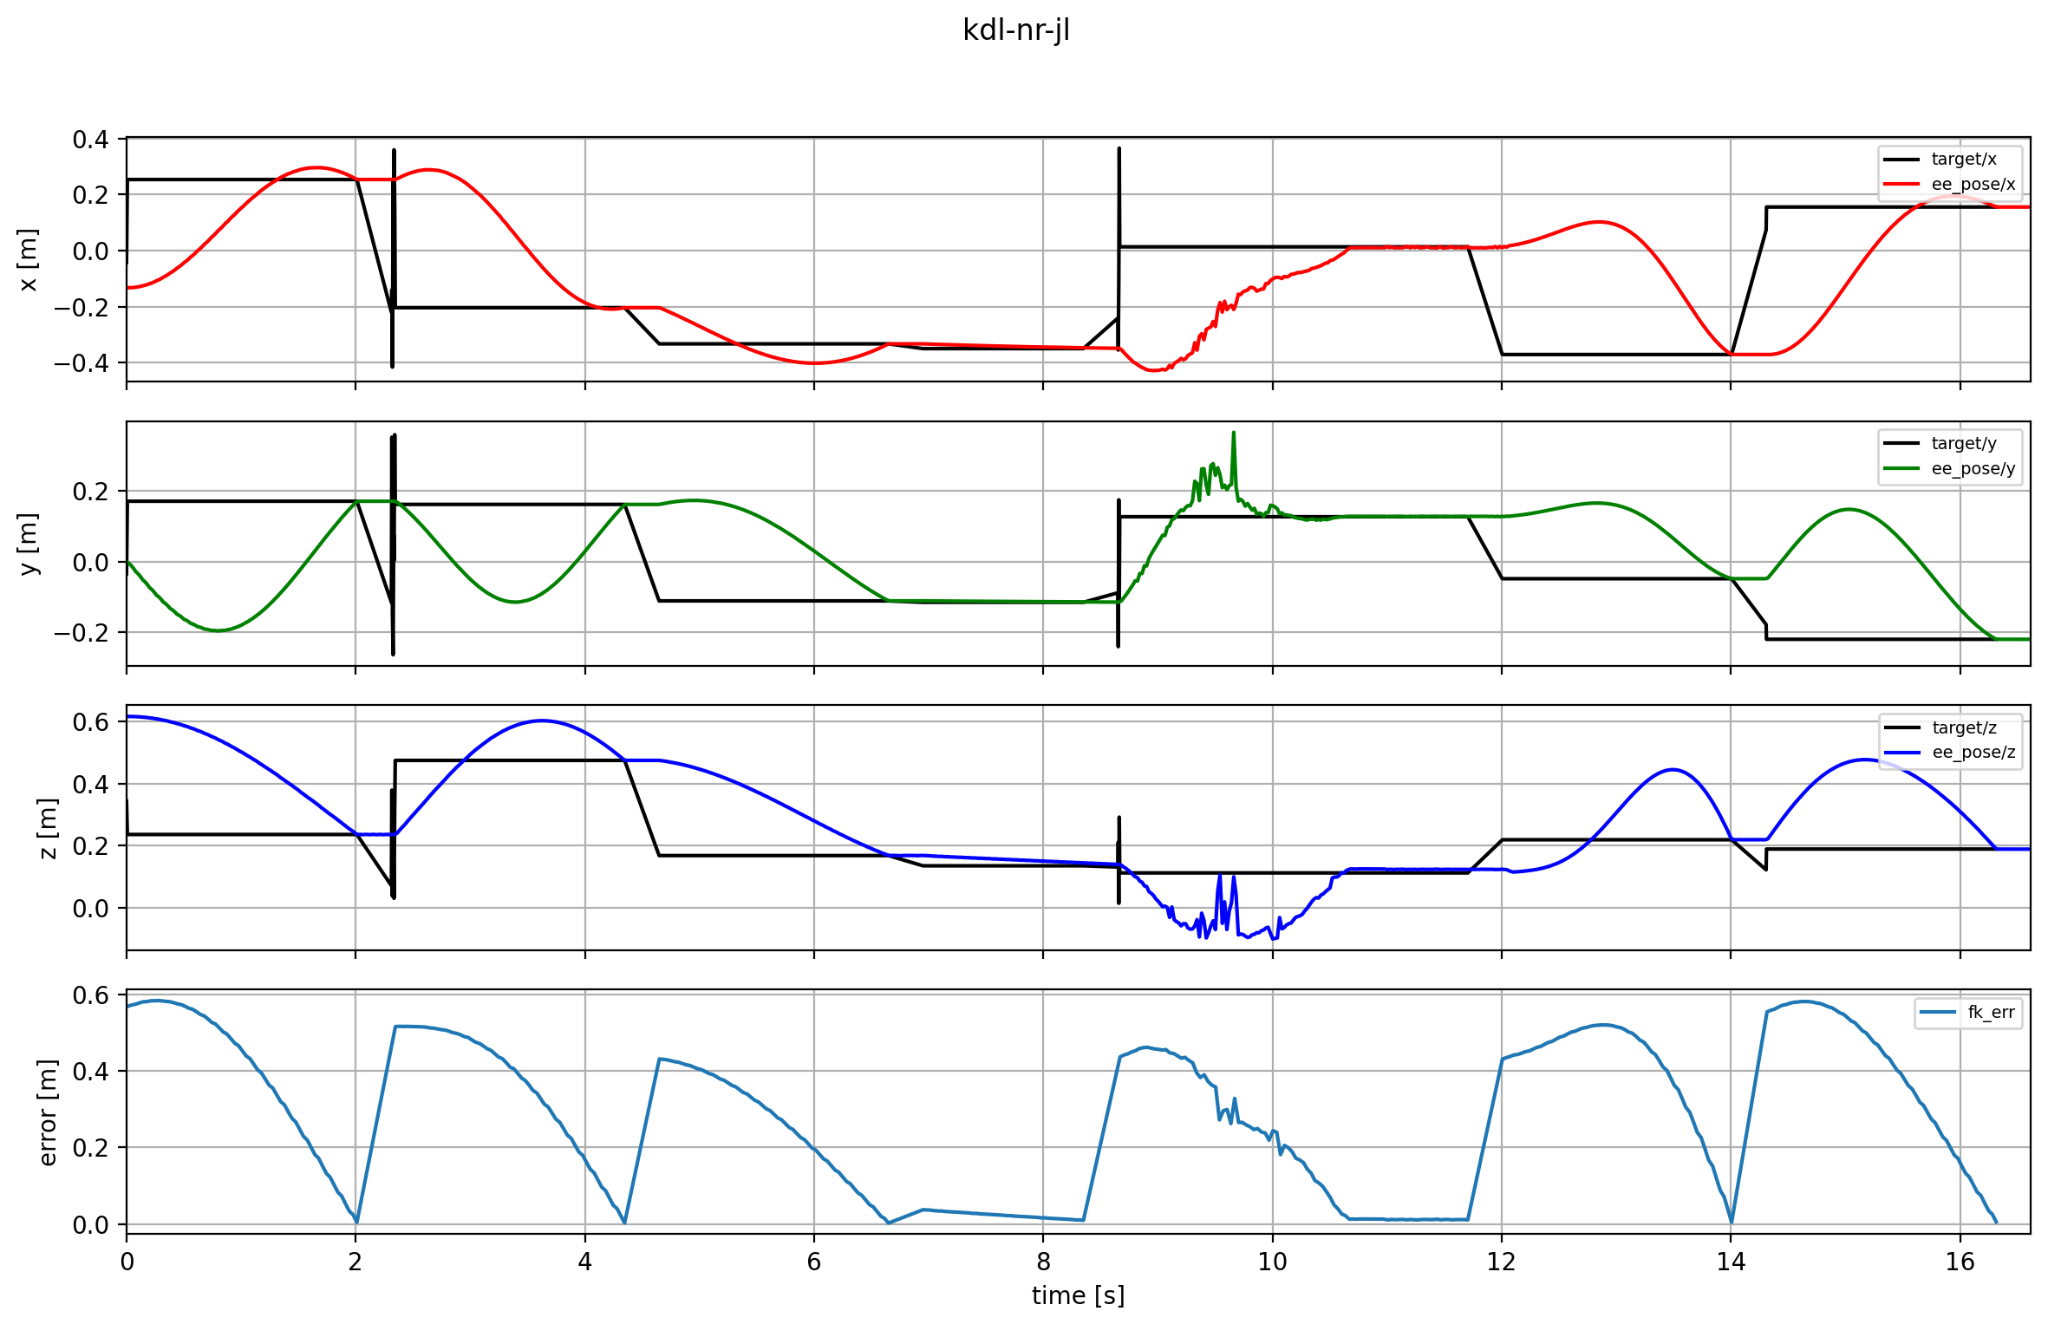
\includegraphics[width=\linewidth]{s05_img03.png}
    \caption{KDL-NR\_JL の例（目標値と追従，誤差）}
  \end{subfigure}
  \caption{各 IK ソルバにおける追従結果例}
  \label{fig:results}
\end{figure}

\section{失敗パターンの整理}
観測された代表的な失敗パターンは以下である．fileciteturn1file0L27-L27
\begin{itemize}
  \item \textbf{IK 失敗によるウェイポイントのスキップ}：特に KDL 系で発生しやすい．
  \item \textbf{収束遅れによる残差誤差}：ステップ入力直後にピークが現れやすい．
  \item \textbf{一時的な追従遅れ}：目標が急変した際に手先が大きく遅れる．
\end{itemize}

\section{考察}
予測していた「精度・総時間・初期姿勢に対するロバスト性」は概ね一致した一方，
「解が得られる確率（到達成功率）」については追加検討が必要である．fileciteturn1file0L30-L30
特に，初期姿勢によって KDL-NR / KDL-NR\_JL の到達数が増えるケースが観測された．fileciteturn1file0L30-L30
これは，最初の実験で用いた「直線的（straight）姿勢」が特異点に入りやすく収束しづらいのに対し，
後の「屈曲（bend）姿勢」では収束しやすく他点への到達可能性が増えたため，
KDL 系の成功率が上昇したと解釈できる．fileciteturn1file0L30-L30

\section{結論と今後の課題}
ROS/Gazebo によるシミュレーションを通して，IK ライブラリ間で挙動が異なり，
条件によって収束性が大きく変化することを確認した．fileciteturn1file0L33-L33
今後の改善として，(i) 実機による検証，(ii) 姿勢を含む到達可能領域（Workspace）の同定，
(iii) フィードバック用センサの付加，などが挙げられる．fileciteturn1file0L33-L33

\section*{参考}
DOBOT Magician E6 製品ページ：\url{https://jp.dobot-robots.com/products/education/magician-e6.html}

\end{document}
""".lstrip()

tex_path = base/"report.tex"
tex_path.write_text(tex, encoding="utf-8")

# zip
zip_path = Path("/mnt/data/robotmanip_report_latex.zip")
with zipfile.ZipFile(zip_path, "w", compression=zipfile.ZIP_DEFLATED) as z:
    z.write(tex_path, arcname="report.tex")
    for fp in fig_dir.glob("*"):
        z.write(fp, arcname=f"figures/{fp.name}")

(zip_path, tex_path)

